\documentclass[border=2pt]{standalone}
\usepackage{tikz}
\begin{document}
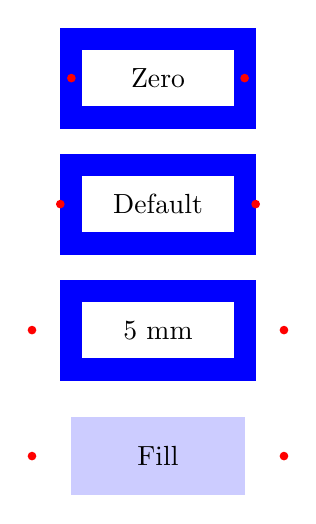
\begin{tikzpicture}[box/.style={rectangle,minimum width=22mm,minimum height=10mm,
                                 inner sep=0pt,line width=8pt,draw=blue,fill=white}]
  \node[box,outer sep=0pt] (zero) at (0,0) {Zero};
  \node[box] (auto) at (0,-1.6) {Default};
  \node[box,outer sep=5mm] (wide) at (0,-3.2) {5 mm};
  \node[box,draw=none,fill=blue!20,outer sep=5mm] (solid) at (0,-4.8) {Fill};
  \foreach \n in {zero,auto,wide,solid}{
    \fill[red] (\n.west) circle[radius=.55mm];
    \fill[red] (\n.east) circle[radius=.55mm];
  }
\end{tikzpicture}
\end{document}
